\documentclass[border=2pt]{standalone}
\usepackage{fontspec}
\setmainfont{Liberation Serif}
\usepackage{tikz,graphicx,pgfplots}
\usetikzlibrary{arrows.meta,positioning,matrix,calc}
\pgfplotsset{compat=1.18}
\definecolor{forest}{HTML}{176044}
\definecolor{sage}{HTML}{EAF4EE}
\definecolor{rulec}{HTML}{CBD4CF}
\definecolor{ink}{HTML}{192723}
\definecolor{warm}{HTML}{F3ECE4}
\tikzset{all/.style={font=\fontsize{10.5pt}{12.5pt}\selectfont,text=ink},
box/.style={all,draw=rulec,fill=sage,rounded corners=2pt,align=center,inner sep=4pt,minimum height=0.9cm},
mutedbox/.style={box,fill=white},warmbox/.style={box,fill=warm},
flow/.style={-{Latex[length=2.4mm]},line width=.65pt,draw=forest}}
\begin{document}
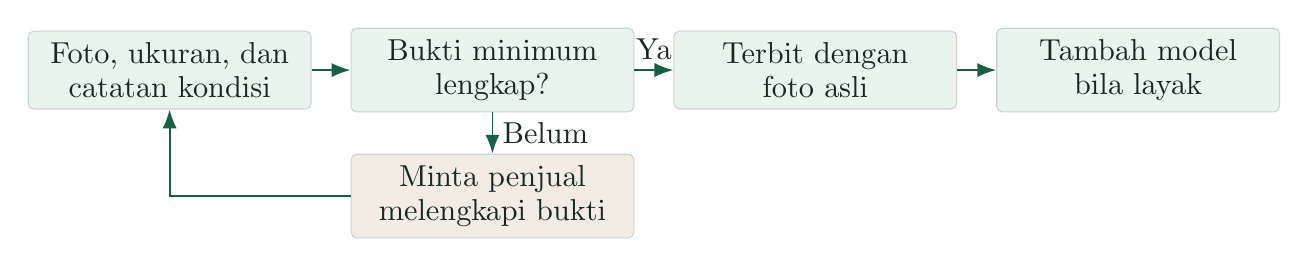
\begin{tikzpicture}[x=1cm,y=1cm]
\node[box,text width=3.31cm] (a) at (1.95,.55) {Foto, ukuran, dan\\catatan kondisi};
\node[box,text width=3.31cm] (b) at (6.05,.55) {Bukti minimum\\lengkap?};
\node[box,text width=3.31cm] (c) at (10.15,.55) {Terbit dengan\\foto asli};
\node[box,text width=3.31cm] (d) at (14.25,.55) {Tambah model\\bila layak};
\node[warmbox,text width=3.31cm] (e) at (6.05,-1.05) {Minta penjual\\melengkapi bukti};
\draw[flow](a)--(b);\draw[flow](b)--node[all,above]{Ya}(c);\draw[flow](c)--(d);
\draw[flow](b)--node[all,right]{Belum}(e);\draw[flow](e.west)-|(a.south);
\end{tikzpicture}
\end{document}
